{\descr{Дослідити функцію на неперервність}}

$$
  f(x) = \left\{
    \begin{array}{cr}
          -x & x \leqslant 0 \\
        -(x-1)^2 & 0 < x < 2 \\
          x-3 & x \geqslant 2 \\
    \end{array}
  \right
$$

1) Сробуємо знайти границі функції зліва та зправа точки $0$ в якій функція не визначена
$$
  \lim_{x\to0 \ -0} -x = 0 \qquad   \lim_{x\to0 \ +0} -(x-1)^2 = -(0-1)^2  = -1
$$

\textbf{Висновок} - функція в точкі $0$ являє собою \textbf{розрив першого роду}, оскільки границі функції зліва та зправа дорівнюють одна одній і є скінченними.

\newline
\
\newline

2) Сробуємо знайти границі функції зліва та зправа точці $2$ (в якій функція не визначена)
$$
  \lim_{x\to2 \ -0} -(x-1)^2 = -(2-1)^2 = -1 \qquad \lim_{x\to2 \ +0} (x-3) = (2-3) = -1
$$

\textbf{Висновок} - функція в точкі $2$ являє собою \textbf{усувний розрив}, оскільки границі функції зліва та зправа не дорівнюють одна одній і є скінченними.

\begin{figure}[h!]
  \centering
  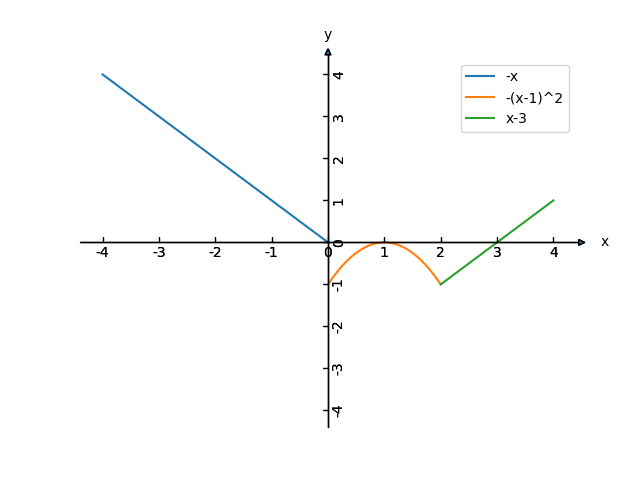
\includegraphics[width=14cm]{rozrahunkova_01/04_01.png}
  \caption{Графік функції}
  \label{fig:rr_01_40_01}
  \centering
\end{figure}
